\documentclass[twocolumn]{aastex62}
\usepackage{bm}
\usepackage{amsmath,amsfonts,amssymb}
\usepackage{color}
\usepackage{comment}
%\usepackage{layouts}

\newcommand\teff{T_{\rm eff}}
\newcommand\logg{\log{g}}
\newcommand\feh{[\rm{Fe}/\rm{H}]}

\newcommand{\project}[1]{\textsl{#1}}
\newcommand{\package}[1]{\texttt{#1}}
\newcommand{\acronym}[1]{{\small{#1}}}
\newcommand{\article}{\emph{Article}}

\newcommand{\Gaia}{\project{Gaia}}
\newcommand{\gaia}{\project{gaia}}
\newcommand{\Galah}{\project{Galah}}
\newcommand{\GALAH}{\project{GALAH}}
\newcommand{\todo}[1]{\textcolor{red}{#1}}


\newcommand{\vect}[1]{\boldsymbol{\mathbf{#1}}}
\renewcommand{\vec}[1]{\vect{#1}}

\newcommand{\weight}{\pi}
\newcommand{\data}{\textbf{Y}}
\newcommand{\vecdata}{\vec\data}

\newcommand{\nextstep}{^\textrm{(t+1)}}
\newcommand{\thisstep}{^\textrm{(t)}}
\newcommand{\transpose}{^\intercal}
\newcommand{\eye}{\textbf{I}}

\newcommand{\factorloads}{\textbf{L}}
\newcommand{\factorscores}{\textbf{S}}
\newcommand{\specificvariance}{\vec{D}}

\newcommand{\scoremeans}{\vec\xi}
\newcommand{\scorecovs}{\vec\Omega}

\newcommand{\NumData}{N}
\newcommand{\NumDimensions}{D}
\newcommand{\numdata}{n}
\newcommand{\numdimensions}{d}
\newcommand{\NumLatentFactors}{J}
\newcommand{\numlatentfactors}{j}
\newcommand{\NumComponents}{K}
\newcommand{\numcomponents}{k}
\newcommand{\likelihood}{\mathcal{L}}



\received{2019 March XX}
\revised{2019}
\accepted{2019}

\newcommand{\vcpath}{vc.tex}

\IfFileExists{\vcpath}{\input{\vcpath}}{
	\newcommand{\giturl}{UNKNOWN}
	\newcommand{\gitslug}{UNKNOWN}
	\newcommand{\githash}{UNKNOWN}
	\newcommand{\gitdate}{UNKNOWN}
	\newcommand{\gitauthor}{UNKNOWN}
}



\submitjournal{AAS Journals}

\shorttitle{Chemical tagging in lower-dimensional latent space}
\shortauthors{Casey et al.}

\begin{document}

\title{Chemical tagging in lower-dimensional latent space}

\correspondingauthor{Andrew R. Casey}
\email{andrew.casey@monash.edu}

\author[0000-0003-0174-0564]{Andrew R. Casey}
\affiliation{School of Physics \& Astronomy, 
			 Monash University,
			 Wellington Rd, Clayton 3800, Victoria, Australia}
\affiliation{Faculty of Information Technology, 
			 Monash University, 
			 Wellington Rd, Clayton 3800, Victoria, Australia}
			 
\author{John Lattanzio}
\affiliation{School of Physics \& Astronomy, 
			 Monash University,
			 Wellington Rd, Clayton 3800, Victoria, Australia}

\author{Aldeida Aleti}
\affiliation{Faculty of Information Technology, 
			 Monash University, 
			 Wellington Rd, Clayton 3800, Victoria, Australia}

\author{David Dowe}
\affiliation{Faculty of Information Technology, 
			 Monash University, 
			 Wellington Rd, Clayton 3800, Victoria, Australia}
			 
\author{the GALAH team}


\begin{abstract}
Chemical tagging promises to distinguish unique star formation sites from 
observed photospheric abundances.
Clustering techniques applied in chemical tagging have to date assumed that
all photospheric abundances are independent, a provably false assumption.
Nucleosynthetic processes make multiple elements in varying quantities, and the
dimensionality of chemical abundance space is typically lower than the 
number of reported abundances. 
Here we introduce a novel approach to chemical tagging where a set of 
latent factors (e.g., nucleosynthetic yields) contribute to the
data, and clustering is performed in the latent space (e.g., relative counts of
nucleosynthetic events). In doing so we infer basis vectors that are analogous
to nucleosynthetic yields, and the lower dimensional latent space allows for
more efficient clustering. We perform experiments on literature chemical abundances
of metal-poor stars, \todo{others}, and 
those from the second \Galah\ data release. \todo{We find that 5 latent factors are
preferred to explain the chemical abundances of metal-poor stars, and 8 are
needed to account for \Galah\ data.}
We describe exact methods and software that scale well with the data,
allowing for chemical tagging experiments for $10^{7.5}$ abundance measurements
to be performed in minutes.
\end{abstract}


\keywords{methods: statistical}

\section{Introduction} \label{sec:intro}

Chemical tagging seeks to identify star formation events using the present
day photospheric abundances of stars \citep{Freeman;Bland-Hawthorn:2002}.
The detailed chemical abundances observable in a star's photosphere provide a
fossil record that carries with it information about where and when a star
formed. While the photospheric abundances remain largely unchanged throughout
a star's lifetime \citep[however see][]{Dotter:2017,Ness:2018b}, the dynamical 
dissipation timescale of open clusters in the Milky Way disc is of order a few 
gigayears \citep{Portegies-Zwart:1998}. That makes chemical tagging an attractive 
approach to identify star formation sites long after those stars are no longer 
gravitationally bound to each other.


Gravitationally bound star clusters have been useful laboratories for
testing the limits and utility of chemical tagging. Although biases arise when
only considering star clusters that are still gravitationally bound, the chemical
homogeneity of open clusters provides an empirical measure of how similar stars
would need to be before they could be tagged as belonging to the same
star formation site \citep{Mitschang:2014}. However, there are also analysis
issues in understanding how well those chemical abundances can be measured
\citep{Bovy:2016}, and how chemically similar multiple unrelated stars (or
doppleg\"angers) can be \citep{Ness:2018}.
If open clusters were truely chemically homogeneous then our
ability to chemically tag the Milky Way depends on the precision with which we
can measure those chemical abundances in stars. Data-driven techniques are
driving a revolution in this field \citep{Ness:2015,Ness:2018a,Ness:2018b,
Casey:2016,Casey:2017,Ho:2017b,Ho:2017a,Leung;Bovy:2018}, but there is more work
to do: astronomers have not yet reached the Cram\'er-Rao bound for chemical 
abundances of stars.


There are further chemical tagging obstacles to overcome once all the chemical 
abundance information in a stellar spectrum can be extracted. Most notably is a 
catalogue of precise detailed chemical abundances for a large number of stars,
where those chemical abundances trace different nucleosynthetic pathways.
This is the primary scientific goal of the \Galah\ survey \citep{DeSilva:2015,Martell:2017,Buder:2018},
a stellar spectroscopic survey that uses the High Efficiency and Resolution 
Multi-Element Spectrograph \citep[\project{HERMES};][]{Sheinis:2015} on the Australian 
Astronomical Telescope (AAT).  \Galah\ will observe up to $10^6$ stars in the 
Milky Way, and measure up to 30 chemical abundances for each star. This includes
light odd-Z elements (e.g., Na, K), elements produced through
alpha-particle capture (e.g., Mg, Ca, Ti), and elements produced
through the slow (e.g., Ba) and rapid neutron-capture process
(e.g., Eu). These data provide an unparalleled view on the production
of chemical elements in the Milky Way.


Given these data and the most
favourable assumptions in chemical tagging -- that star clusters are truely
chemically homogenous, and we can measure those abundances with infinite precision,
and those abundances are differentiable between star clusters -- then chemical
tagging becomes a clustering problem. All clustering techniques applied to 
chemical tagging assume that the data dimensions are independent. That is to say
that adding a dimension of [Ni/H] provides totally new, independent information.
Theory and observations agree that this cannot be true.
Nucleosynthetic processes produce multiple elements in varying
quantities, and the dimensionality of stellar abundance datasets has been shown
to be lower than the actual number of dimensions \citep{Ting:2012, Price-Jones:2018}.
Any clustering approach that treats each new elemental abundance as an 
independent axis of information will therefore conclude with biased inferences
about the star formation history of our Galaxy. 


Alternative approaches are perhaps more challenging, as it is difficult to prescribe
the nucleosynthetic yields that have contributed to the chemical abundances of each star
with great confidence. There are
qualitative statements that can be made for large numbers of stars, or particular
types of stars, but quantifying the precise contribution of different processes
to each star is an unsolved problem. For example, the [$\alpha$/Fe] `knee' in
abundance ratios in the Milky Way can qualitatively be explained by 
core-collapse supernovae being the predominant nucleosynthetic process in the
early Milky Way before Type Ia contributions had a significant impact, but 
efforts to date have not sought to try to explain the detailed abundances of a 
single star as a contribution of yields from different systems (e.g., 20\% of the
Ba was produced by 3 M$_\odot$ systems). This is in part because of the
challenging and degenerate nature of the problem as described, and is complicated
by the differences in yield predictions that account from prescriptions used in
different codes.


New approaches to chemical tagging are clearly needed. Immediate advances would
include methods that take the dependence among chemical elements into account
within some generative model, or techniques that combine chemical abundances
with dynamical constraints to place joint prior probabilities on whether any
two stars could have formed from the same star cluster, given some model of the
Milky Way. In this work we focus on the former. Here we present a new approach
to chemical tagging that allows us to identify the latent (unobserved) factors
that contribute to the chemical abundances of all stars (e.g., nucleosynthetic
yields) while simultaneously performing clustering in the latent space.
Notwithstanding caveats that we will
discuss in detail, this allows us to infer nucleosynthetic yields rather than
strictly prescribe them from models. Moreover, the scale of the clustering
problem reduces by a significant fraction because the clustering is performed in
a lower dimensional latent space instead of the higher dimensional data space.
In Section~\ref{sec:methods} we describe the model and the methods we use to
estimate the model parameters. Section~\ref{sec:experiments} describe the 
experiments performed using generated and real data sets. We discuss the results
of these experiments in Section~\ref{sec:discussion}, including the caveats with
the model as described. We conclude in Section~\ref{sec:conclusion}.



\section{Methods} \label{sec:methods}

Factor analysis is a common statistical approach for describing correlated 
observations with a lower number of latent variables \citep[e.g.,][]{Thompson:2004}.
Related techniques include principal component analysis \citep{Hotelling:1933} and its
variants \citep{Tipping;Bishop:1999}, singular value decomposition \citep{Golub:1970}, and other
matrix factorization methods. While factor analysis on its own is a useful
dimensionality reduction tool to identify latent factors that contribute to
the chemical abundances of stars \citep[e.g.,][]{Price-Jones:2018}, factor
analysis cannot describe clustering in the data (or latent) space.
Similarly, clustering techniques applied to chemical abundances to date 
\citep[e.g.,][]{Hogg:2016} do not account for the lower dimensionality of the
data. 

Here we expand on a variant of factor analysis known elsewhere as a mixture of common 
factor analyzers \citep{Baek:2010}, where the data are generated by a set of 
latent factors that are common to all data, but the scoring (or extent) of those
factors is different for each data point, and the data can be modelled as a
mixture of multivariate normal distributions in the latent space (factor scores).
In this work the data $\vecdata$ is a 
$\NumData \times \NumDimensions$ matrix where $\NumData$ is the number of 
stars and $\NumDimensions$ is the number of chemical abundances measured 
for each star. We assume a generative model for the data 
\begin{equation}
	\vecdata = \factorloads\factorscores + \vec{e}
	\label{eq:generative-model}
\end{equation}

\noindent{}where $\factorloads$ is a $\NumLatentFactors \times \NumDimensions$ 
matrix of factor loads that is common to all data points, and the factor scores 
for the $\numdata$th data point
\begin{equation}
	\factorscores_\numdata \sim \mathcal{N}(\vec\xi_\numcomponents, \vec\Omega_\numcomponents)
\end{equation}
\noindent{}are drawn from the $\numcomponents$th multivariate normal distribution.
The factor scores for all data points $\factorscores$ is then a 
$\NumData \times \NumLatentFactors$ matrix, where each data point has a partial
association to the components in latent space. 
We assume $\vec{e} \sim \mathcal{N}\left(\vec{0}, \eye\specificvariance\right)$
is independent of the latent space, and $\specificvariance$ is a
column vector of $\NumDimensions$ entries. 
In this model each data point can be represented as being drawn
from a mixture of multivariate normal components, except the components
are \emph{clustered in the latent space} $\factorscores$ and projected
into the data space by the factor loads $\factorloads$. 


We assume that the latent space is lower dimensionality than the
data space (e.g., $\NumLatentFactors < \NumDimensions$).
Within the context of stellar abundances, the factor loads
$\factorloads$ can be thought of as the \emph{typical} yields
of nucleosynthetic
events (e.g., $s$-process production from AGB stars), and the
factor scores are analogous to the relative counts of those 
nucleosynthetic events. The clustering in factor scores
achieves the same as a clustering procedure in data space,
except we simultaneously estimate the latent processes that are
common to all stars (the so-called factor loads, analogous to 
nucleosynthetic yields). Within this framework a rare nucleosynthetic event
can still be described as a `factor load' $\factorloads_\numlatentfactors$, 
but its rarity would be represented by associated factor
scores being zero for most stars and thus have negligible contribution
to the observed abundances. In practice the factor loads can only be 
identified up to orthogonality and cannot be expressly interpreted as
nucleosynthetic yields because they have limited physical meaning
(we discuss this further in Section~\ref{sec:discussion}),
but this description of typical yields and relative event rates should
help build intuition for the model parameters, and provide context
within the astrophysical problem it is being applied.


Including latent factors in the model description allows us to account for 
processes that affect multiple elemental abundances. In this way we are 
accounting for the fact that the data dimensions are not independent of
each other. Another benefit is the scaling with computational cost. If we 
considered data sets of order $10^{7.5}$
entries (e.g., 30 chemical abundances for $10^6$ stars) purely as a
clustering problem, then even the most efficient clustering
algorithms would incur a significant cumulative computational 
overhead by searching the parameter space for the number of
clusters, and the optimal model parameters given that number
of components. However, because the mixture of factor analyzers
approach assumes that there is a \emph{lower dimensional latent 
space} in which the data are clustered, and that clustering is 
projected into real space by common factor loads, the 
dimensionality of the clustering problem is reduced from 
$N \times D$ to $N \times J$. This reduces computational cost through
faster execution of each optimization step, and on average fewer optimization steps
needed to reach a specified convergence threshold.

From a statistical standpoint, the primary advantage to using
a mixture of factor analysers is that we can simultaneously
estimate latent factors (e.g., infer nucleosynthetic 
yields) and perform clustering (e.g., chemical tagging) 
within a statistically consistent framework. That is to say
that we have a generative model for the data that can 
quantitatively account for nucleosynthetic yields, variations in
turbulence and gas mixing, or star formation efficiency,
and the parameters of this model can be estimated consistently
given some data.

Without loss of generality the density of the data $\vecdata$ can be described as
\begin{equation}
	f(\vecdata; \vec\Psi) = \sum_{\numcomponents=1}^{\NumComponents}\weight_\numcomponents\phi(\vecdata;\factorloads\scoremeans_\numcomponents, \factorloads\scorecovs_\numcomponents\factorloads\transpose + \eye\specificvariance)
\end{equation}
\noindent{}given $\NumLatentFactors$ common factor loadings and $\NumComponents$ components
clustered in the latent (factor score) space. Here the parameter
vector
$\vec\Psi$ includes $\{\factorloads,\vec\pi,\scoremeans,\scorecovs,\specificvariance\}$, and $\phi(\vecdata;\vec\mu, \vec\Sigma)$
describes the density of a multivariate gaussian distribution with
mean $\vec\mu$ and covariance matrix $\vec\Sigma$,
and $\weight_\numcomponents$ describes the relative weighting of the $\numcomponents$th
component in latent space and $\sum\weight_\numcomponents = 1$.
The log likelihood is then given by
\begin{equation}
	\log\mathcal{L}(\vecdata|\vec\Psi) = \sum_{\numcomponents=1}^{\NumComponents}\log{f(\vecdata;\vec\Psi)} \quad . \label{eq:log-likelihood}
\end{equation}


As mentioned previously, the model as described is indeterminate in that
there is no unique solution for the factor loads $\factorloads$ and scores
$\factorscores$. These quantities can only be determined up until 
orthogonality in $\factorloads$. However, as we will show, accurate estimates
of the parameter vector $\vec\Psi$ can be obtained by the expectation-maximization
algorithm \citep{Dempster:1977}. 
% TODO: say something about "..with a suitable number of initial guesses?"


\subsection{Initialisation}

Here we describe the default initialisation of the model parameters, which
we have found to be robust in a large set of models. Given a number of
$\NumLatentFactors$ latent factors we initialise the factor load
$\factorloads$ entries to be drawn from a uniform distribution
$\factorloads \sim \mathcal{U}\left(-1, +1\right)$ and then ensure that
the factor loads are orthogonal such that
%TODO: Should we re-write this so that we just draw from the scipy special ortho group?
\begin{equation}
	\factorloads \factorloads\transpose = \eye \quad .
\end{equation}
We then initially assign each data point as belonging to one of the
$\NumComponents$ components by drawing from a multinomial distribution
and generating the $\NumData \times \NumComponents$ responsibility matrix $\vec\tau$,
where $\sum_{k=1}^{K} \tau_{nk} = 1$ for any $n$th row. Given the initial
factor loads and assignments, we then estimate the relative weights
$\vec\pi$, the mean factor scores of each component $\scoremeans$, and
the covariance matrix of factor scores of each component $\scorecovs$.
Finally, we initialise the specific variance $\specificvariance$ in each
dimension as the variance in each data dimension. Other initialisation 
methods are available in the code associated with this \emph{Article}. 
Throughout this work we found that the optimised model parameters are 
insensitive to the choice of initialisation, up until orthogonal 
rotation of the latent space.


\subsection{Expectation-Maximization}

We use the expectation-maximization algorithm to estimate the model parameters
\citep{Dempster:1977}. With each expectation step we evaluate the log likelihood 
given the model parameters $\vec\Psi$, and we re-calculate the $\NumData \times \NumComponents$ responsibility 
matrix $\vec\tau$ whose entries are the posterior probability that the 
$\numdata$th data point is associated to the $\numcomponents$th component, given 
the data $\vecdata$ and the current estimate of the parameter vector $\vec\Psi$:
\begin{equation}
	\tau_{\numdata\numcomponents} = \frac{\weight_\numcomponents\phi(\vecdata_\numdata;\factorloads\scoremeans_\numcomponents, \factorloads\scorecovs_\numcomponents\factorloads\transpose + \eye\specificvariance)}{\sum_{g=1}^{G}\weight_g\phi(\vecdata_\numdata;\factorloads\scoremeans_g, \factorloads\scorecovs_g\factorloads\transpose + \eye\specificvariance)} \quad .
\end{equation}


At the maximization step we update our estimates of the parameters,
conditioned on the data $\vecdata$ and the responsibility matrix $\vec\tau$.
The updated parameters estimates are found by setting the second derivative
of the log-likelihood (Eq.~\ref{eq:log-likelihood}) to zero and solving for
the parameter values. In doing so this guarantees that every updated
estimate of the model parameters is guaranteed to increase the log-likelihood.
Although there are no guarantees against converging on local minima, in 
general it is sufficient to run expectation-maximization from multiple
initialisations in order to ensure that the global minima is reached.
At the maximization step we first update our estimate of the relative weights 
$\vec\weight\nextstep$ given the responsibility matrix $\vec\tau$
\begin{equation}
	\weight_\numcomponents\nextstep = \frac{1}{\NumData} \sum_{\numdata=1}^{\NumData}\tau_{\numdata\numcomponents}
	% Include proof.
\end{equation}
\noindent{}where the $\vec{X}\thisstep$ superscript refers to the current estimate of a variable
and $\vec{X}\nextstep$ refers to the updated estimate for the next iteration.


The updated estimates of the mean factor scores 
$\scoremeans\nextstep$ for each component are then given by
\begin{eqnarray}
	\scoremeans_\numcomponents\nextstep = \scoremeans_\numcomponents\thisstep + \frac{\vec{G}\transpose(\vecdata\transpose - \factorloads\thisstep\scoremeans_\numcomponents\thisstep)\vec\tau_\numcomponents}{\NumData\weight_\numcomponents\nextstep}
\end{eqnarray}
\noindent{}where:
\begin{eqnarray}
	\vec{W} &=& (\scorecovs_\numcomponents\thisstep)^{-1}\eye \\
	\vec{V} &=& \left(\specificvariance\thisstep\right)^{-1} \\
	\vec{C} &=& (\vec{W} + (\factorloads\thisstep)\transpose\vec{V}\factorloads\thisstep)^{-1}\eye \\
	\vec{G} &=& \left[\vec{V} - \vec{V}\factorloads\thisstep\vec{C}\left(\vec{V}\factorloads\thisstep\right)\transpose\right]\factorloads\thisstep\scorecovs_k\thisstep \quad .
\end{eqnarray}

The covariance matrices of the components of factor scores $\scorecovs\nextstep$
are updated next,
\begin{equation}
	\scorecovs_\numcomponents\nextstep = \left(\eye - \vec{G}\transpose\factorloads\thisstep\right)\scorecovs_\numcomponents\thisstep + \frac{\vec{G}\transpose\vec{Z}\left(\vec{Z}\vec\tau_\numcomponents\transpose\right)\transpose\vec{G}}{N\weight_\numcomponents\nextstep}
\end{equation}
\noindent{}where
\begin{eqnarray}
	\vec{Z} &=& \vecdata\transpose - \factorloads\thisstep\scoremeans_\numcomponents\thisstep \quad .
\end{eqnarray}

After some linear algebra, updated estimates of the common factor loads $\factorloads\nextstep$
can be found from
\begin{equation}
	\factorloads\nextstep = \factorloads_{1}\left(\factorloads_{2}^{-1}\eye\right)
\end{equation}
\noindent{}where:
\begin{eqnarray}
	\factorloads_1 &=& \sum_{\numcomponents=1}^{\NumComponents}\left[ \vec\tau_\numcomponents\transpose\vecdata\left(\scoremeans_\numcomponents\thisstep\right)\transpose + 
	\vec{G}\transpose\vec\tau_\numcomponents\vec{Z}\transpose\vec{G}\right] \\
	\factorloads_2 &=& N\sum_{\numcomponents=1}^{\NumComponents}\left[\weight_\numcomponents\nextstep\left(\scorecovs_\numcomponents\nextstep + \scoremeans_\numcomponents\nextstep\left(\scoremeans_\numcomponents\nextstep\right)\transpose\right)\right]
\end{eqnarray}


Finally, the updated estimate of the specific variances $\specificvariance\nextstep$ is given
by
\begin{equation}
	\specificvariance\nextstep = \frac{1}{\NumData}\left[\sum^{\NumComponents}_{\numcomponents=1}\vec\tau_\numcomponents\transpose\left(\vecdata\odot\vecdata\right) - \sum_{j=1}^{J}\left(\factorloads\nextstep\factorloads_2\right)\odot\factorloads\nextstep\right]
\end{equation}

\noindent{}where $\odot$ denotes is the entry-wise (Hadamard) product. We repeat
the expectation-maximization cycle for up to 10,000 steps or until the log-likelihood
improved by less than $10^{-5}$ between successive iterations. Although our implementation
allows for a positive regularisation term to be added along the diagonal of the covariance
matrices in latent space $\scorecovs$, we set this regularisation term to zero for all
experiments performed here.



\begin{figure*}
	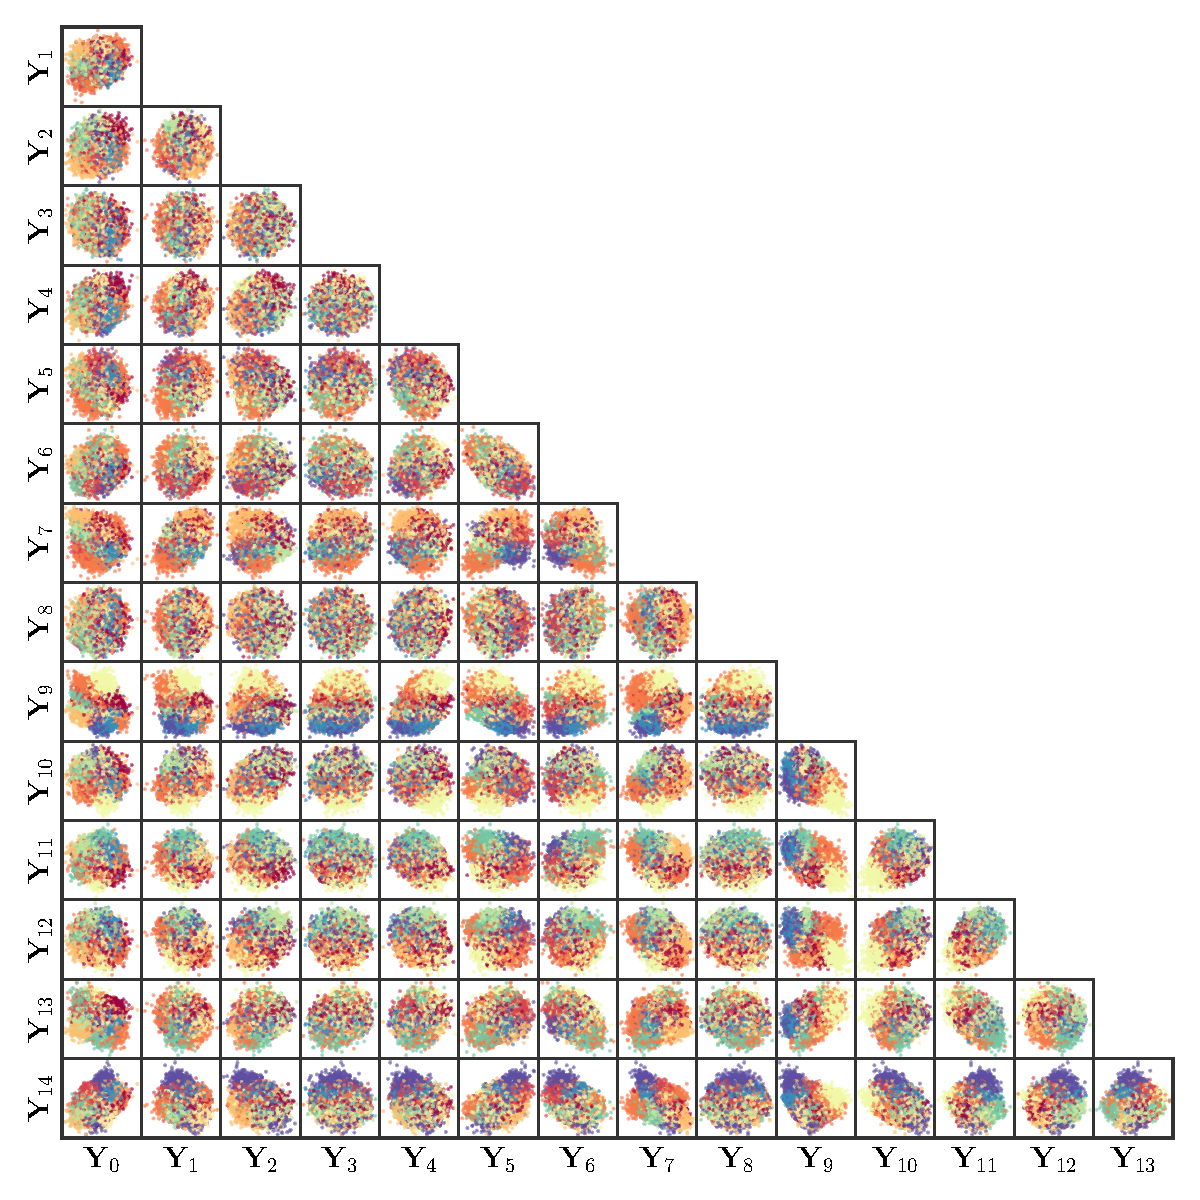
\includegraphics[width=1.0\textwidth]{experiments/exp1-data-colour.pdf}
    \caption{The generated data for Experiment~1, where points are coloured by their
		     true associations to each component.}
    \label{fig:exp1-data}
\end{figure*}


\subsection{Model Selection}

The expectation-maximization algorithm as described requires the number of latent
factors $\NumLatentFactors$ and $\NumComponents$ to be given. In the next Section
we describe experiments using generated and real data, and in all cases we will
assume that the true number of latent factors and components are not known. 
We require some criterion to decide how many latent factors, and how many
components, we should adopt given some data. An increasing number of factors
and components will undoubtedly increase the log likelihood of the model given
the data, but the log likelihood does not account for the increased model 
complexity that is afforded by those additional latent factors and components.


One criterion commonly employed for evaluating a class of models is the 
Bayesian Information Criterion \citep[BIC;][]{Schwarz:1978}, 
\begin{equation}
	\textrm{BIC} = Q\log{N} - 2\log\mathcal{L}\left(\data|\vec\Psi\right) \quad , \label{eq:bic}
\end{equation} 
\noindent{}where $Q$ is the number of model parameters:
\begin{equation}
	Q = \frac{\NumLatentFactors}{2}\left[2\left(\NumDimensions - \NumLatentFactors\right) + \NumComponents\left(3 + \NumLatentFactors\right)\right] + \NumComponents + \NumDimensions - 1 \quad .
\end{equation}
\noindent{}We evaluate the BIC for all experiments performed in this work.
However, while the BIC does include a penalisation term for the number of
parameters (which scales with $\log{N}$), it does not account for the increased
complexity that is afforded by additional parameters. Adding one parameter
to a model will increase the BIC by at most $\log{N}$, but there are different
ways for a single parameter to be introduced. In a fictitious model $y=f(x)$
a parameter $b$ could be added that is a scalar multiple of $x$, or it could be
introduced as $x^b$. Despite the difference in model complexity, the same
penalisation occurs in BIC. Even if the log likelihood were only to improve
marginally in both cases, the difference in model complexity is not captured
by BIC. In other words, there are situations where we are more interested in
balancing the model complexity (or the expected Fisher information and similar
properties) with the goodness of fit, instead of penalising the number of 
parameters.


For these reasons we also calculate the Minimum Message Length \citep[MML;][]{Wallace:2005}
for every model as a criterion for model selection and evaluation. 
The classically-described princple of MML is that the best explanation of the
data is the one that leads to the shortest so-called two-part message~\cite{Wallace:2005}, 
where a \textit{message} takes into account both the complexity of the model 
and its explanatory power. The complexity of the model is described through
the first part of the message, and the second part of the message describes
its explanatory power. The \emph{length} of each message part is quantified
(or measured) using information theory, allowing for a fair evaluation between
different models of varying complexity or explanatory power. MML has been 
shown to perform well on a variety of empirical analyses (see, e.g., 
\cite{viswanathan1999finding,fitzgibbon2004minimum}, with references to 
further examples in \cite{Wallace:2005,dowe2007bayes,Dowe2008a,Dowe2011a}).
Arguments about the statistical consistency (i.e.,~as the number of data 
points increases the distributions of the estimates become increasingly 
concentrated near the true value) of MML are given in \cite{DoweWallace1997a,Dowe2011a}.
The MML principle requires that we explicitly specify our prior beliefs on the
model parameters, providing a Bayesian optimisation approach which can be
applied across entire classes of models.

The \textit{message} must encode two parts: the model, and the data given the
model. The encoding of the message is based on Shannon's information theory~\cite{Shannon:1948}. 
The information gained from an event $e$ occurring, where $p(e)$ is the
probability of that event, is $I(e) = -\log_{2}{p(e)}$. The information content
is largest for improbable outcomes, and smallest for outcomes that we are 
almost certain about. In other words, an outcome that has a probability close
to unity has zero information content because nothing new is learned from it,
whereas rarer events convey a much higher information content. 

In practice calculating the message length can be a non-trivial task, 
especially for models that are reasonably complex. This makes the strict MML
principle intractable (or uncomputable) in many cases and necessitating 
approximations to the message length. Using a Taylor expansion, a generalised
scheme can be calculated to estimate the parameter vector $\vec\Psi$ that
minimises the message length ${I}(\vec\Psi,\vecdata)$ \citep{Wallace:1987},
\begin{equation}
	{I}(\vec\Psi,\vecdata) = \frac{Q}{2}\log\kappa_q - \log\left(\frac{p(\vec\Psi)}{\sqrt{|\mathcal{F}(\vec\Psi)|}}\right) - \log\mathcal{L}\left(\vecdata|\vec\Psi\right) + \frac{Q}{2} \label{eq:mml} 
\end{equation}
\noindent{}where $\log\likelihood(\vecdata|\vec\Psi)$ is the familiar
log likelihood, $p(\vec\Psi)$ is the joint prior density on $\vec\Psi$,
$\mathcal{F}(\vec\Psi)$ is the negative second derivative of the log likelihood,
commonly referred to as the expected Fisher information matrix,
\begin{equation}
	\mathcal{F}(\vec\Psi) = -\textrm{E}\left[\frac{\partial^2}{\partial\vec\Psi^2}\log\likelihood(\vecdata|\vec\Psi)\right]
\end{equation}
\noindent{}and as before $Q$ is the number of model parameters.
Continuous parameters can only be stated to finite precision, which leads
to the $\frac{Q}{2}\log\kappa_q$ term that gives a measure of the volume of the region of
uncertainty in which the parameters $\vec\psi$ are centred. The $\log\kappa_q$
term is
\begin{equation}
	\log\kappa_q = -\log{2\pi} + \frac{1}{Q}\log{Q\pi} - \gamma - 1
\end{equation}
\noindent{}where $\gamma$ is Euler's constant.

Like the BIC, the message length is penalised by the number of model parameters
through the $\log\kappa(Q)$ term. However, the model complexity is also 
described through the priors and the Fisher information matrix, which
describes the curvature of the log likelihood with respect to the model
parameters. 

%\todo{Dowe said something about MML reducing to BIC under some conditions, but I have not yet found the right paper to cite.}


We will describe the contributions to the message length in parts. We assume
the priors on the number of latent factors $\NumLatentFactors$ and the
number of components $\NumComponents$ to be
$p(\NumLatentFactors) \propto 2^{-\NumLatentFactors}$ and
$p(\NumComponents) \propto 2^{-\NumComponents}$ respectively,
such that the optimal lossless message to encode them is \citep[p279, sec. 6.8.2][]{Knorr-Held:2000},
\begin{eqnarray}
	I(\NumLatentFactors) &= -\log{p(\NumLatentFactors)} &= \NumLatentFactors\log{2} + \textrm{constant} \label{eq:prior_J} \\
	I(\NumComponents) &= -\log{p(\NumComponents)} &= \NumComponents\log{2} + \textrm{constant} \label{eq:prior_K} \quad .
\end{eqnarray}
Only $\NumComponents - 1$ of the relative weights $\vec\weight$ need encoding because 
$\sum_{\numcomponents=1}^{\NumComponents} = 1$. We assume a uniform prior on 
individual weights,
\begin{equation}
	p(\vec\weight) = (\NumComponents - 1)! \quad ,
\end{equation}
\noindent{}and the Fisher information is
\begin{equation}
	\mathcal{F}(\vec\weight) = \frac{\NumData^{\NumComponents - 1}}{\prod_{\numcomponents=1}^{\NumComponents}\weight_\numcomponents} \quad ,
\end{equation}
\noindent{}which gives the message length of the relative weights $I(\vec\weight)$ to be
\begin{eqnarray}
	I(\vec\weight) &=& -\log\left(\frac{p(\vec\weight)}{\sqrt{|\mathcal{F}(\vec\weight)|}}\right) \nonumber \\
			   &=& -\log{p(\vec\weight)} - \frac{1}{2}\log{|\mathcal{F}(\vec\weight)|} \nonumber  \\
			   &=& -\log(\NumComponents - 1)! + \frac{\NumComponents - 1}{2}\log{\NumData} - \frac{1}{2}\sum_{\numcomponents=1}^{\NumComponents}\log\weight_\numcomponents \nonumber \\
	I(\vec\weight) &=& \frac{1}{2}\left(\left(\NumComponents - 1\right)\log\NumData - \sum_{\numcomponents=1}^{\NumComponents}\log\weight_\numcomponents\right) -\log\Gamma(\NumComponents) \quad . \nonumber \label{eq:prior_pi} \\
\end{eqnarray}

We assume uniform priors for the component means in latent space $\scoremeans$, 
and a conjugate inverted Wishart prior for the component covariance matrices
$\scorecovs$ \citep[Section 5.2.3][]{Knorr-Held:2000},
\begin{equation}
	p(\scoremeans_\numcomponents,\scorecovs_\numcomponents) \propto |\scorecovs_\numcomponents|^{\frac{1}{2}(\NumLatentFactors + 1)} \quad .
\end{equation}
We approximate the determinate of the Fisher information of a multivariate normal $|\mathcal{F}(\scoremeans,\scorecovs)|$
as $|\mathcal{F}(\scoremeans)||\mathcal{F}(\scorecovs)|$ \citep{Oliver:1996,Figueiredo:2002} where
\begin{equation}
	|\mathcal{F}(\scoremeans)| = (\NumData\weight_k)^\NumLatentFactors|\scorecovs_k|^{-1}
\end{equation}
\begin{equation}
	|\mathcal{F}(\scorecovs)| = (\NumData\weight_k)^{\frac{1}{2}\NumLatentFactors(\NumLatentFactors+1)}2^{-\NumLatentFactors}|\scorecovs_k|^{-(\NumData+1)}
\end{equation}
\noindent{}such that 
% todo put line in equation.
\begin{eqnarray}
	I(\scoremeans,\scorecovs) &=& -\sum_{\numcomponents=1}^{\NumComponents}\log{p(\scoremeans_k,\scorecovs_k)} + \frac{1}{2}\sum_{\numcomponents=1}^{\NumComponents}\log{|\mathcal{F}(\scoremeans_k,\scorecovs_k)|} \nonumber \\
	&=& \frac{1}{2}\sum_{\numcomponents=1}^{\NumComponents}\log\left[(\NumData\weight_k)^{\frac{1}{2}\NumLatentFactors(\NumLatentFactors+3)}2^{-\NumData}|\scorecovs_k|^{-(\NumData + 2)}\right] \nonumber \\
	&& \cdots \,\, -\sum_{\numcomponents=1}^{\NumComponents}\log{|\scorecovs_k|}^{\frac{1}{2}(\NumLatentFactors + 1)} \\
I(\scoremeans,\scorecovs) &=& \frac{1}{4}\NumLatentFactors(\NumLatentFactors+3)\sum_{\numcomponents=1}^\NumComponents\log{\NumData\weight_k} - \frac{KD}{2}\log{2} \nonumber \\ 
&& \cdots \,\, -\frac{1}{2}(2\NumLatentFactors+3)\sum_{k=1}^{K}\log{|\scorecovs_k|}  \quad . \label{eq:prior_xi_omega} 
\end{eqnarray}

Previous work on multiple latent factor analysis within the context of MML have
addressed the indeterminacy between the factor loads and factor scores by
placing a joint prior on the product of factor loads and scores, whilst
ensuring that the factor loads themselves remain mutually orthogonal \citep{WallaceMLF}.
Adopting the same prior density in our model is not practical because 
it would require priors on $\scoremeans$, $\scorecovs$, and the 
responsibility matrix $\vec\tau$. Instead, we address this indeterminacy
by placing a prior on $\factorloads$ that ensures it is mutually orthogonal.
Specifically, we adopt a Wishart distribution with scale matrix $\vec{S}$
and $D$ degrees of freedom for the
$\NumLatentFactors\times\NumLatentFactors$ matrix $\vec{M} = \factorloads\transpose\factorloads$.
In other words, $\vec{M} \sim W_\NumLatentFactors(D,\vec{S})$
and $\vec{S} = \textrm{Cov}(\factorloads\transpose)$.
This
Wishart joint prior density gives highest support for mutually orthogonal vectors,
\begin{equation}
	p(\factorloads) = \frac{|\factorloads\transpose\factorloads|^{\frac{1}{2}(\NumDimensions - \NumLatentFactors - 1)}}{2^{\frac{\NumDimensions\NumLatentFactors}{2}}|\vec{S}|^{\frac{\NumDimensions}{2}}\Gamma(\frac{\NumDimensions}{2})}\exp\left[-\frac{1}{2}\textrm{Tr}(\vec{S}^{-1}\factorloads\transpose\factorloads)\right] \quad .
\end{equation}
The Fisher information for $\factorloads$ \todo{is hard to compute. I have 
the first derivative from the log likelihood function, but the second
derivative is (surprisingly) causing some trouble to compute.}
Thus the message length to encode $\factorloads$ is given by
\begin{eqnarray}
	I(\factorloads) &=& -\log\left(\frac{p(\factorloads)}{\sqrt{|\mathcal{F}(\factorloads)|}}\right) \nonumber \\
	&=& -\log{p(\factorloads)} + \todo{\frac{1}{2}\log{|\mathcal{F}(\factorloads)|}} \nonumber \\
I(\factorloads)	&=& \frac{1}{2}\textrm{Tr}(\textrm{Cov}(\factorloads\transpose)^{-1}\factorloads\transpose\factorloads) - \frac{1}{2}(\NumDimensions - \NumLatentFactors - 1)\log{|\factorloads\transpose\factorloads|} \nonumber \\
	&& \cdots \,\, + \frac{1}{2}\NumDimensions\NumLatentFactors\log{2} + \frac{1}{2}\NumDimensions\log{|\textrm{Cov(\factorloads)}|} - \Gamma\left(\frac{\NumDimensions}{2}\right) \quad .\nonumber \label{eq:prior_L} \\
\end{eqnarray}

Combining equations \ref{eq:prior_J}, \ref{eq:prior_K}, \ref{eq:prior_pi}, \ref{eq:prior_xi_omega}, and \ref{eq:prior_L} with equation \ref{eq:mml} leads to the full message length
\begin{eqnarray}
	I(\vec\Psi, \vec\data) &=& -\log\likelihood(\vec\data|\vec\Psi) \nonumber \\
	&& +\frac{1}{4}\left(\NumLatentFactors + 4\right)\left(\NumLatentFactors - 1\right)\sum_{\numcomponents=1}^\NumComponents\log\weight_\numcomponents + \left(\NumComponents - \frac{1}{2}\right)\log{\NumData} \nonumber \\
	&& +\frac{1}{2}\NumDimensions\log|\textrm{Cov}\left(\factorloads\transpose\right)| - \frac{1}{2}\left(D-J-1\right)\log|\factorloads\transpose\factorloads| \nonumber \\
	&& +\textrm{Tr}\left(\textrm{Cov}\left(\factorloads\transpose\right)^{-1}\factorloads\transpose\factorloads\right) - \left(\NumLatentFactors + \frac{3}{2}\right)\sum_{\numcomponents=1}^\NumComponents\log|\scorecovs_\numcomponents| \nonumber \\
	&& -\log\Gamma\left(\NumComponents\right) - \Gamma\left(\frac{\NumDimensions}{2}\right) + \frac{Q}{2}\log\kappa_q \nonumber \\
	&& +\frac{1}{2}\left[\NumLatentFactors(\NumDimensions + 2) + \NumComponents(2-\NumData)\right]\log{2} \quad .
\end{eqnarray}




% -\log\likelihood(\vec\data|\vec\Psi) \
% + (J + K + \frac{KN}{2} + \frac{DJ}{2})\log{2}     --> \frac{1}{2}(3(J+K) + ND)\log{2}
% 0.5*((K-1) logN - \sum\log\weight)  + \frac{1}{4}J(J+3)\sum\log(N\weight) --> 
% -\log\gamma(K) - \Gamma(D/2)
% -\frac{1}{2}(2J+3)\sum\log|\omega_k|
% + factor loads stuff
% + Q/2\log\kappa(q)
 





\clearpage

\section{Experiments} \label{sec:experiments}




\subsection{Experiment 1: Toy model with generated data} \label{sec:experiment-toy-model}




We generated a data set with ${\NumData = 1}$00,000 data points, each with
$\NumDimensions = 15$ dimensions. We adopted a latent dimensional space of 
$\NumLatentFactors = 5$ ($\NumLatentFactors \times \NumDimensions$) factor loads, 
with $\NumComponents = 20$ clusters in the latent space. The relative weights $\vec\weight$
are drawn from a multinomial distribution and the means of the clusters
in factor scores $\scoremeans$ are drawn from a standard normal
distribution. The off-diagonal entries in the covariance matrices in factor scores $\scorecovs$ are drawn from a gamma distribution $\scorecovs_{\numcomponents,i,i} \sim \vec\Gamma\left(1\right)$. The variance in 
each dimension $\specificvariance$ are also drawn $\specificvariance \sim \vec\Gamma\left(1\right)$.
We randomly draw a  $\NumDimensions \times \NumDimensions$ matrix from a Haar distribution \citep{Haar:1933},
which is uniform on the special orthogonal group $\textrm{SO}(n)$ and therefore guaranteed to return an orthogonal
matrix with a determinant of unity \citep{Stewart:1980}.
We denote the $\NumLatentFactors \times \NumDimensions$ left-most region of this
matrix to be $\mathbf{H}$, and by taking $\factorloads_\ast$ to be the Cholesky decomposition of $\mathbf{H}\transpose \mathbf{H}$, we find the factor loads
\begin{eqnarray}
 	\factorloads = \mathbf{H}\left(\left(\factorloads_\ast\right)^{-1}\eye\right)
\end{eqnarray}
\noindent{}which ensures that the true factor loads is a $\NumLatentFactors \times \NumDimensions$
matrix of mutually orthogonal vectors and that $\factorloads\transpose \factorloads = \eye$.
The $\numdata$th data point (which belongs to the $\numcomponents$th cluster) is then
generated by drawing $\factorscores_{\numdata} \sim \mathcal{N}(\scoremeans_\numcomponents,\scorecovs_\numcomponents)$, projecting by the factor loads $\factorloads$, and adding variance $\specificvariance$.




\begin{figure}
	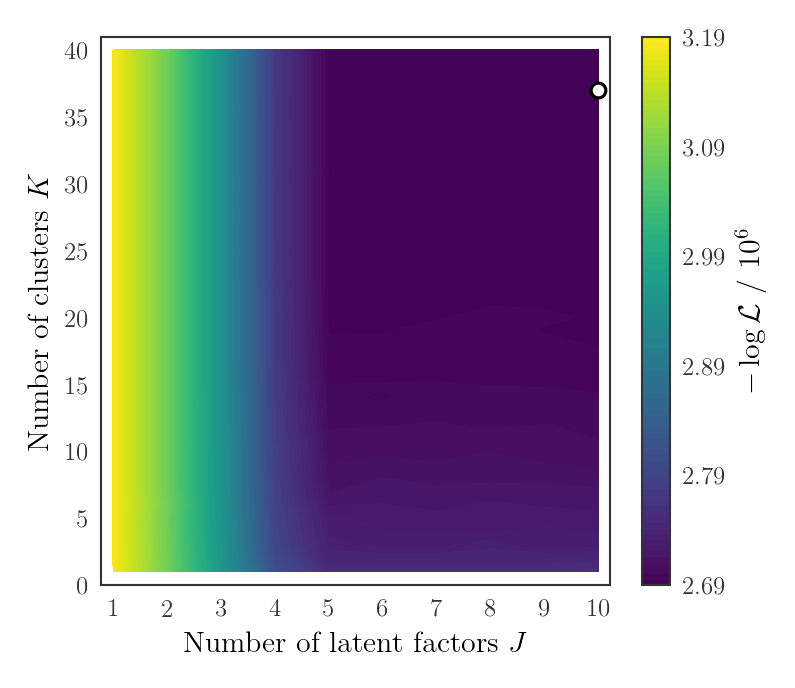
\includegraphics[width=0.45\textwidth]{experiments/exp1-gridsearch-ll-contours.png}
	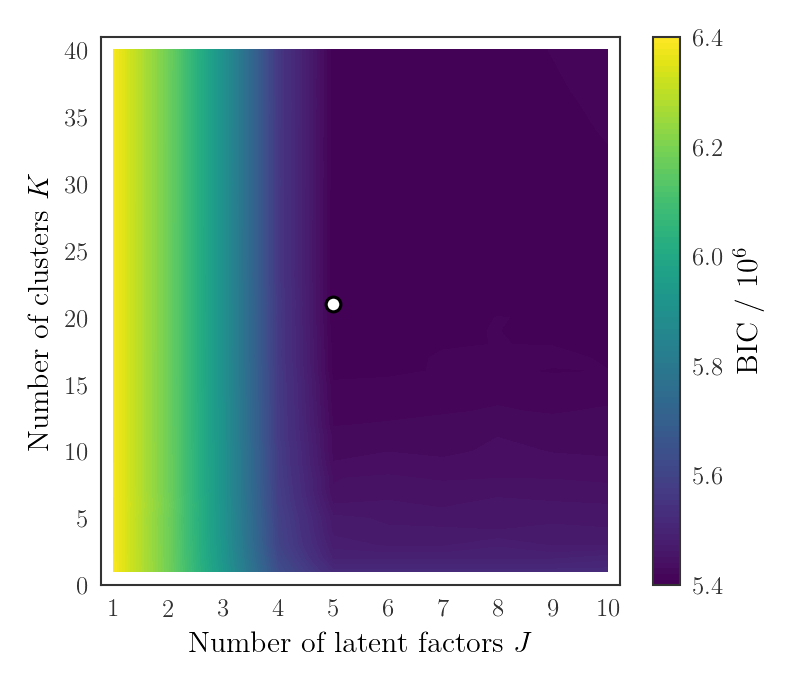
\includegraphics[width=0.45\textwidth]{experiments/exp1-gridsearch-bic-contours.png}
	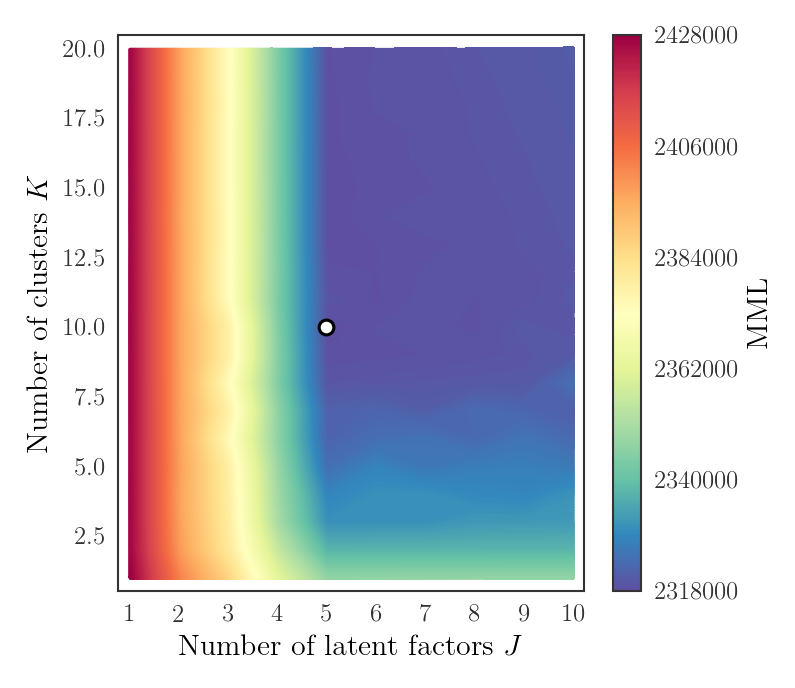
\includegraphics[width=0.45\textwidth]{experiments/exp1-gridsearch-mml-contours.png}
    \caption{Model performance metrics resulting from a gridsearch using the
    		 data generated as part of our toy model. The top 
		 	 panel shows the negative log-likelihood 
			 $-\log{\mathcal{L}\left(\data|\vec\Psi\right)}$ 
			 evaluated at each combination of latent factors $J$ and number 
			 of clusters $K$, and the bottom panel shows the BIC (Equation \ref{eq:bic}).
			 The white marker indicates the 
			 lowest value in each panel, which is joined by a black line from the true value
			 in the top panel. The model with the lowest message length and lowest BIC has
			 the same number of latent factors and components used to generate the data.
		}
    \label{fig:experiment-1-gridsearch}
\end{figure}



Here we treat the generated data set as if the true number of latent factors
and the true number of components are not known. Starting with $\NumLatentFactors = 1$
and $\NumComponents = 1$, we trialled each permutation of $\NumLatentFactors$ and $\NumComponents$
until $\NumLatentFactors_{max} = 10$
and   $\NumComponents_{max} = 40$ (e.g., twice $\NumLatentFactors_\textrm{true}$ and $\NumComponents_\textrm{true}$).
For each $\NumLatentFactors$, $\NumComponents$ permutation we initialised the factor
loads and component assignments randomly. We performed expectation-maximization 
cycles until the relative log-likelihood improved by less than $10^{-5}$. 



These metrics are shown in Figure~\ref{fig:experiment-1-gridsearch}.
Unsurprisingly the log likelihood increases with increasing numbers of latent
factors $\NumLatentFactors$ and increasing numbers of components $\NumComponents$.
The lowest BIC value is found at $\NumLatentFactors = 5$
and $\NumComponents = 20$, identical to the true values.

\begin{figure*}
	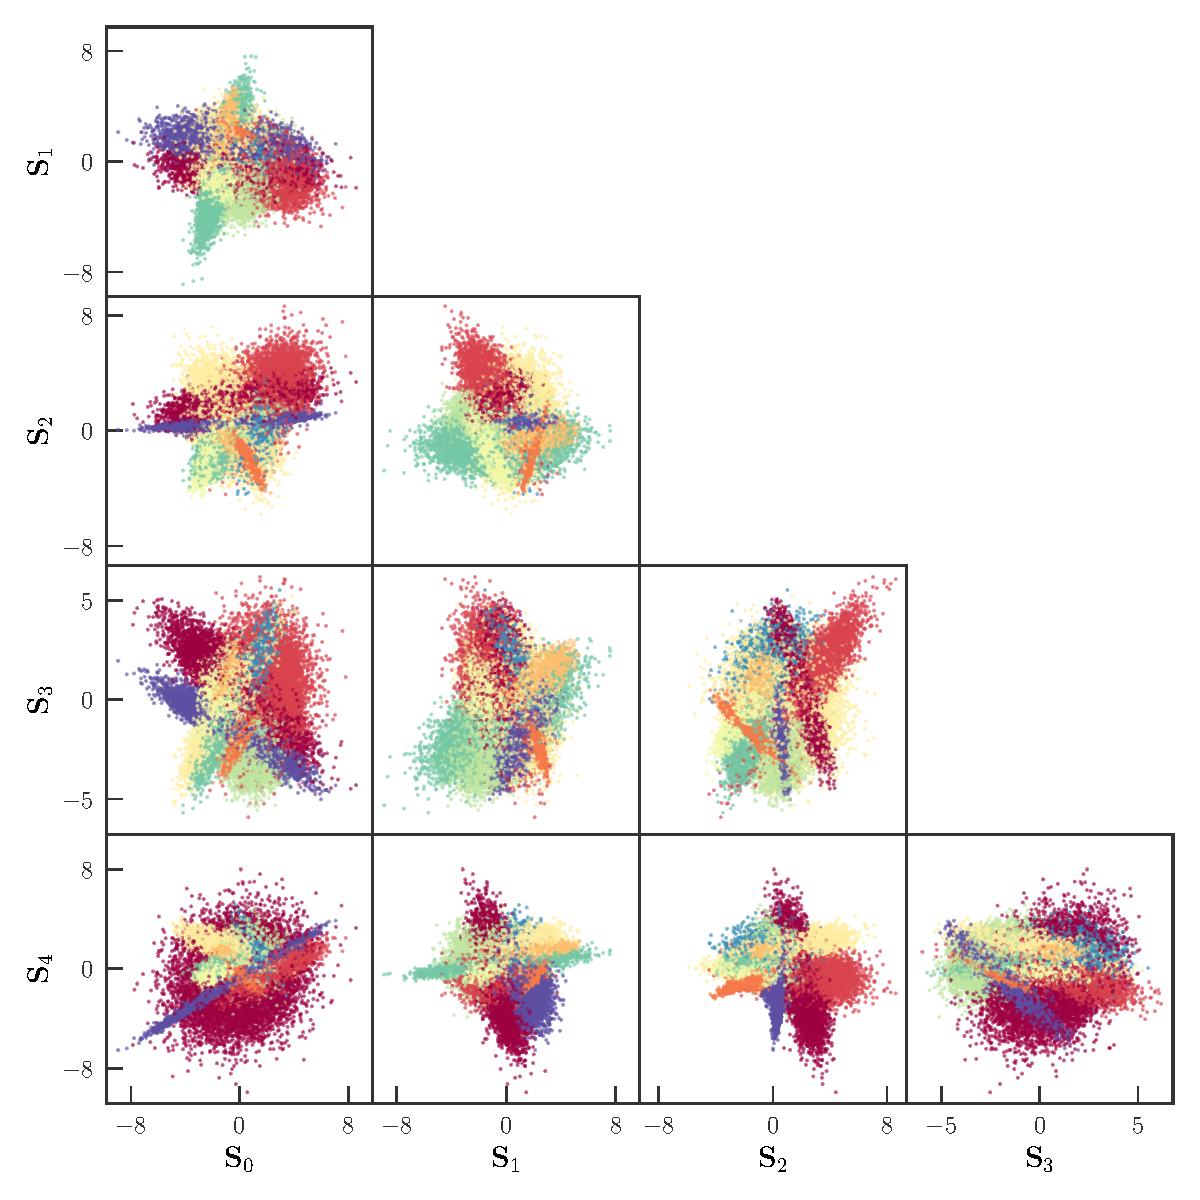
\includegraphics[width=\textwidth]{experiments/exp1-latent.pdf}
    \caption{The inferred latent scores $\factorscores$ for Experiment~1
    		 from a model with $\NumLatentFactors = 5$ latent factors and
		 	 $\NumComponents = 20$ multivariate normal components in
			 latent space.
             Points are coloured by the inferred component.}
    \label{fig:exp1-latent}
\end{figure*}


We show a corner plot of the generated data in Figure~\ref{fig:exp1-data},
demonstrating the clustering (colour) and structure varying structure in data space.
Despite this clustering in data space, it is clear from Figure~\ref{fig:experiment-1-gridsearch} that a combination of latent factors
and allowing clustering in the latent space provides a better description of the data.
Adding components to the model improves the log-likelihood, even with a single latent factor,
but the addition of just one latent factor improvers the log-likelihood more than adding
20 clusters. Not much can be said for this example because the true data generating process 
is drawn from a higher number of latent factors, but this does illustrate how 
clustering in high dimensional data can be better described by latent factors with 
clustering in the lower dimensional latent space.
The inferred clustering in latent space is shown in Figure~\ref{fig:exp1-latent},
where each point is coloured by the inferred associated component. 


\begin{figure*}
	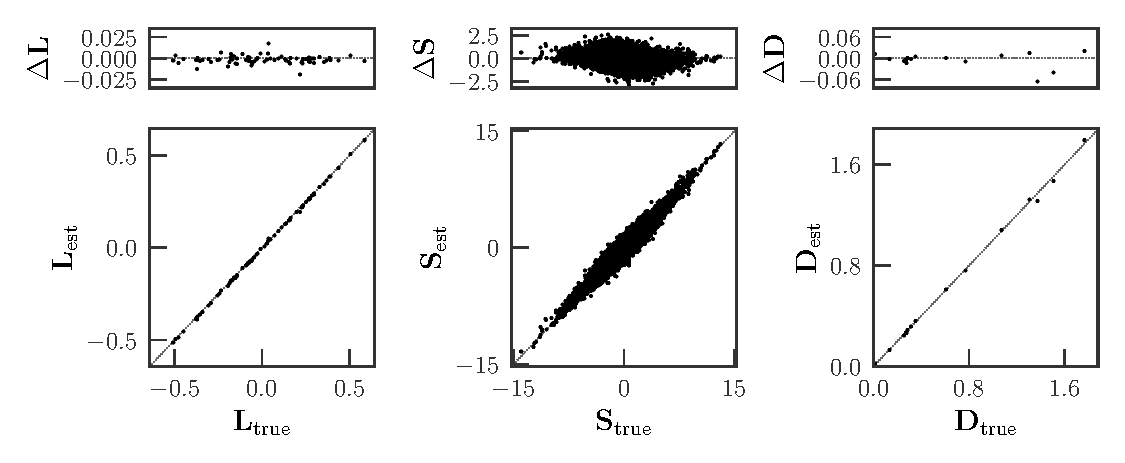
\includegraphics[width=\textwidth]{experiments/exp1-compare-all.pdf}
    \caption{The estimated factor loads $\factorloads$ (left), factor scores $\factorscores$ (middle),
    		 and specific variances $\specificvariance$ (right) compared to the 
		 	 true data generating values
		 	 for Experiment~1. The agreement is excellent.}
    \label{fig:exp1-compare}
\end{figure*}



Some technical discussion is warranted before we compare our estimated model
parameters to the true values. The latent factors in this model are only
identifiable up to an orthogonal rotation. That is to say that
if the data were truely generated by latent factors $\factorloads_\textrm{true}$,
then our estimates of those latent factors $\factorloads_\textrm{est}$ do not need
to be identical to the true values. For example, the ordering of the estimated factors
could be different from the true factors, and the ordering of the dimensionality
in latent space would be correspondingly different. Since no constraint is
placed on the ordering of the factor loads during expectation-maximization,
there is no assurance (or requirement) that our factor loads match the true factor loads.





Another possibility is that the estimated factor loads could be flipped in sign 
relative to the true factor loads, and the scores would similarly be flipped. 
In both of these situations (reordering or flipped signs) the log likelihood 
given the data and the estimated factor loads $\factorloads_\textrm{est}$ 
%\citep[or Kullback-Leibler divergence;][]{Kullback:1951}
would be identical to the log likelihood given the data and the true factor loads 
$\factorloads_\textrm{true}$
despite the difference in ordering and sign. These examples serve to illustrate a more 
general property that the factor loads and factor scores can be orthogonally 
rotated by \emph{any valid rotation matrix}\footnote{A rotation matrix is valid if 
$\vec{R}\vec{R}\transpose = \vec{I}$} $\vec{R}$. The estimated factor loads 
$\factorloads_\textrm{est}$ could therefore appear very different from the true 
values, but they only differ by an orthogonal rotation. 




We took the model with the preferred number of latent factors and components found
from a grid search ($\NumComponents = 20$, $\NumLatentFactors = 5$; which are also
the true values) and applied an orthogonal rotation to the latent space to be as
close as possible to the true values. The rotation matrix $\mathbf{R}$ was found
by solving for $\NumLatentFactors$ unknown angle parameters, each of which is used
to construct a Givens rotation matrix, and then we take the product of those Givens
matrices. This process reduces to Euler angle rotation in three or fewer dimensions.
This process rotates the latent space
($\factorloads$, $\scoremeans$, $\scorecovs$), but has no effect on the model's 
predictive power: the log-likelihood \citep[or the Kullback-Leibler divergence;][]{Kullback:1951} under the
rotated model is indistinguishable from the unrotated model.
In Figure~\ref{fig:exp1-compare} we show the estimated factor loads $\factorloads$,
factor scores $\factorscores$, and specific variances $\specificvariance$ compared
to the true values. The agreement is excellent in all model parameters. 

 


\subsection{Experiment~2:\\Inferring astrophysically realistic latent factors}

In this experiment we use detailed chemical abundances of metal-poor stars 
\citep{Barklem:2005} to demonstrate the utility and limitations
in interpreting the latent factors as nucleosynthetic processes. The data 
can be described as 14 chemical abundance measurements from 61 stars ($\NumData = 61$, $\NumDimensions = 14$), and those 14 chemical elements trace multiple nucleosynthetic pathways. Specifically the chemical
abundances measured include Al (light odd-Z), Mg and Ca ($\alpha$-process), Sc, Ti, Cr, Mn, Fe, Co, and Ni (Fe-peak elements), as well as Sr, Y, Ba, and Eu ($s$/$r$-process). 

We performed a grid search for the optimal number of latent factors 
$\NumLatentFactors$ and components $\NumComponents$, starting from 
$\NumLatentFactors = 1$ and $K = 1$, and trialling up until 
$\NumLatentFactors = 7$ and $\NumComponents = 5$. 
We found that models with higher numbers of latent factors were unable to
converge without adding a regularization constant to the diagonals of the
covariance matrices $\scorecovs$ in latent space. Although it is common
to add a regularization term to the diagonals of covariance matrices
when performing expectation-maximization, we found that our existing
grid search boundaries were sufficient to find the preferred $\NumLatentFactors$
and $\NumComponents$, and chose not to add any regularization term.

We initialised
the model parameters randomly for each permutation of $J$ and $K$, and continued
the expectation-maximization algorithm
until a convergence threshold of $10^{-5}$ was reached in the log likelihood. 
In Figure~\ref{fig:exp2-gridsearch-contours} we show the negative log likelihood 
and BIC recorded for the optimised set of model parameters for each permutation 
of $J$ and $K$. The lowest BIC value is found for $J = 5$ and $K = 1$, indicating
five latent factors are preferred, with no clustering.






Using our preferred model with $J = 5$ and $K = 1$, we sought to find a
rotation matrix that would allow us to identify plausible astrophysical
processes in the factor loads.
Although having to perform this rotation is not comforting, there is utility in
trying to identify the latent factors because the factors can only be rotated by
some valid rotation matrix. That is to say that we will not only exactly what
we have put in: the rotated factors will simply be the closest set of factor
loads that are consistent with the data, allowing us to identify the factor
loads that are astrophysically plausible. We constructed
a $J \times D$ astrophysical factor load matrix $\factorloads_\textrm{A}$ where
all entries were zero except for the following entries:
\begin{itemize}
	\item the entry corresponding to Al in the first latent factor to represent
		  odd-Z element production,
	\item the entries corresponding to Ca and Mg in the second latent factor to
		  represent $\alpha$ particle production,
	\item the entries corresponding to Ni, Co, Fe, Mn, Cr, Ti, and Sc in the third
		  latent factor to represent the Fe-peak group,
	\item the entries corresponding to Sr, Y, and Ba in the fourth latent factor
		  to represent products of the slow neutron capture process, and
	\item the entries corresponding to Eu in the fifth latent factor to represent
		  products of the rapid nucleosynthesis process.
\end{itemize}
These entries were set to $1/\sqrt{E}$ where $E$ is the number of non-zero entries
in that latent factor, in order to ensure that $\factorloads_\textrm{A}$ is
mutually orthogonal. We then found the valid rotation matrix $\vec{R}$ that most
closely approximated the astrophysical loads $\factorloads_\textrm{A}$.
In Figure~\ref{fig:exp2-factor-loads} we show the rotated factor loads found by our
preferred model, and illustrate the relative contributions (positive or negative)
to each element.


\begin{figure}
	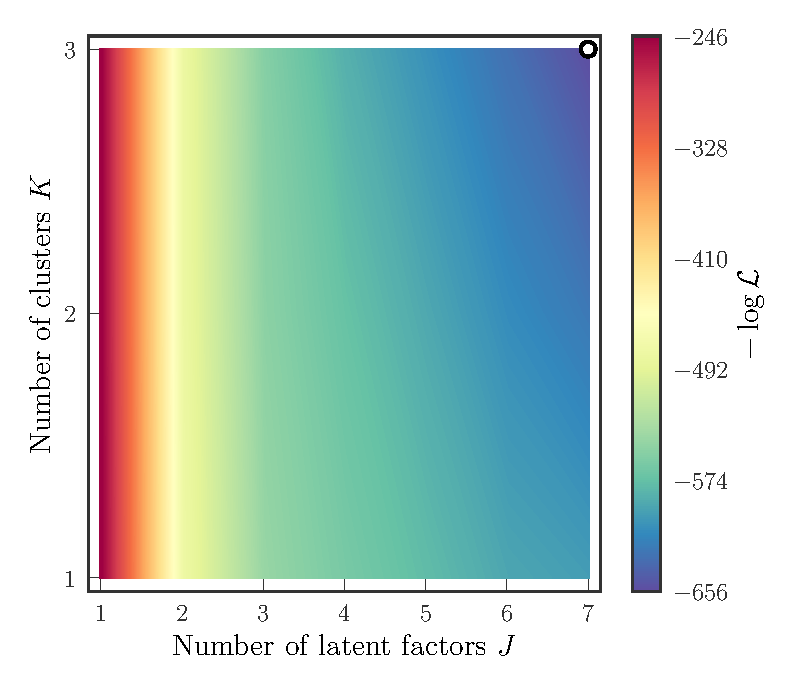
\includegraphics[width=0.45\textwidth]{experiments/exp2-gridsearch-ll.pdf}
	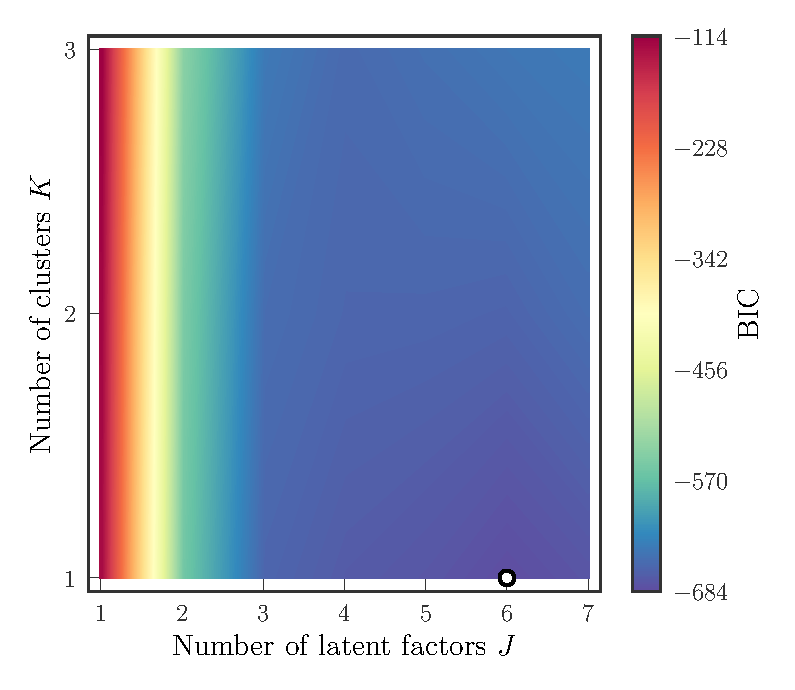
\includegraphics[width=0.45\textwidth]{experiments/exp2-gridsearch-bic.pdf}
    \caption{Model performance metrics resulting from a gridsearch using the
    		 \citet{Barklem:2005} data in Experiment~2.
    		 The top panel shows the negative log-likelihood 
			 $-\log{\mathcal{L}\left(\data|\vec\Psi\right)}$ 
			 evaluated at each combination of latent factors $\NumLatentFactors$ and number 
			 of clusters $\NumComponents$, and the lower panel shows the BIC (Eq.~\ref{eq:bic}).
			 %The cross at
			 %$\NumLatentFactors=8$ and $\NumComponents=5$ indicates that the model could not converge without
			 %adding a regularisation constant to the diagonals of $\scorecovs$.
			 The marker indicates the lowest value in each panel, showing that
			 $\NumLatentFactors = 5$ and $\NumComponents = 1$ is preferred by BIC.}
    \label{fig:exp2-gridsearch-contours}
\end{figure}


The rotated loads are not precisely the same as the target astrophysical loads
in part because the target loads only seek to \emph{identify} and \emph{order}
factors that can be interpreted within an astrophysical context. 
\todo{For example,
the first factor does show positive contributions to Al, like the target load,
but it also shows a slight negative contribution with respect to alpha elements
(Mg, Ca)}, and a gradual increase among Fe-peak elements up to Ni. Similarly while
Ca and Mg are indeed positive in the second factor, as targeted, there is a
weak negative contribution to Mn abundances, which was not part of the target
loads. The fourth factor shows a positive contributions to Sr, Y, Ba, and to a
lesser extent, Eu, which is representative of slow neutron capture production.
Similarly, the last component shows a very strong positive contribution towards
Eu, and could be interpreted as production from the rapid nucleosynthesis process.

\begin{figure*}
	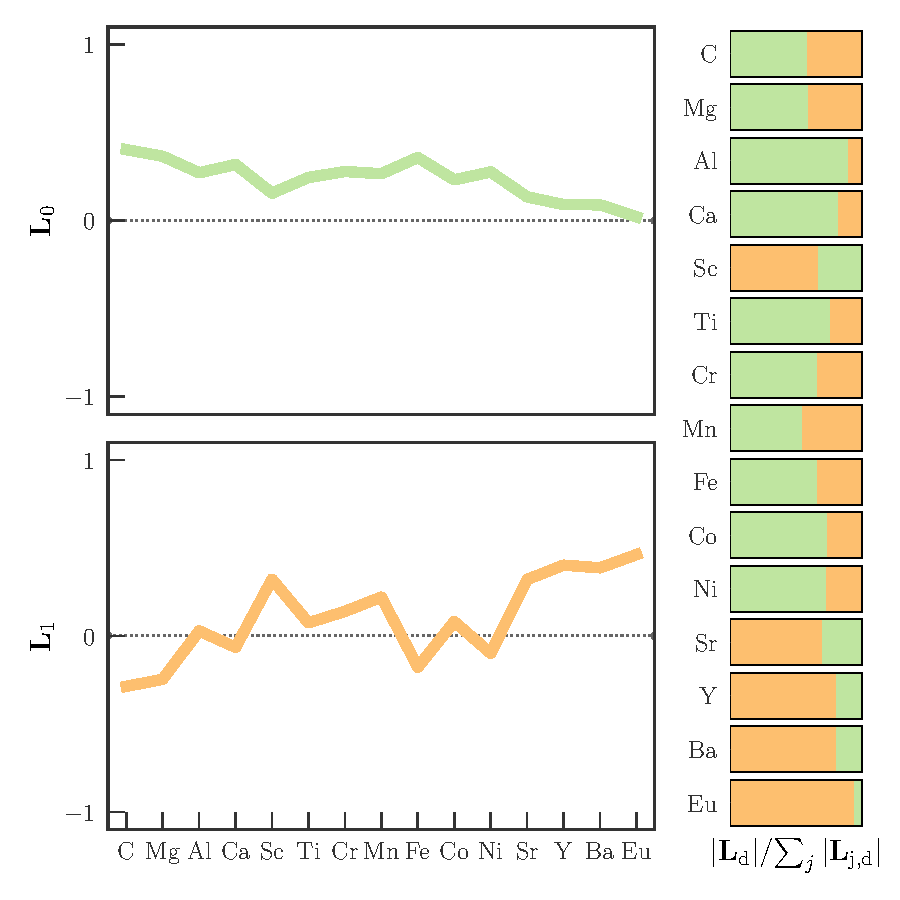
\includegraphics[width=\textwidth]{experiments/exp2-latent-factors-visualize.pdf}
	\caption{Rotated latent factors found in Experiment~2 using the \citet{Barklem:2005}
			 data. The panels on the left show the entries for each factor load. On
			 the right hand side we show the absolute fractional contributions to
			 each element, which illustrates the loads that contribute most to each
			 element (either by positive or negative factor loads).}
    \label{fig:exp2-factor-loads}
\end{figure*}



After accounting for the contributions by all
$J = 5$ factors, the specific scatter remaining in each dimension is shown in
Figure~\ref{fig:exp2-specific-scatter}. The remaining scatter varies from as low 
as 0.08~dex (Mn, Y) up to 0.40~dex (Al, Ba, Ni). Al is not found to have any 
predominant factor in these data: it has non-zero contributions from all loads
(Figure~\ref{fig:exp2-factor-loads}. A similar pattern is seen in Cr, Co, and Ni,
although the specific scatter for Cr and Co is half that of what is found for
Ni (0.2\,dex instead of 0.4\,dex).

% TODO: anything else to say here?



%The relatively wide uncertainty regions on these factors is perhaps not
%surprising given that only 61 stars were used in this data set. However, this
%experiment hopefully demonstrates that the rotated latent factors have some
%interpretability. 



\begin{figure}
	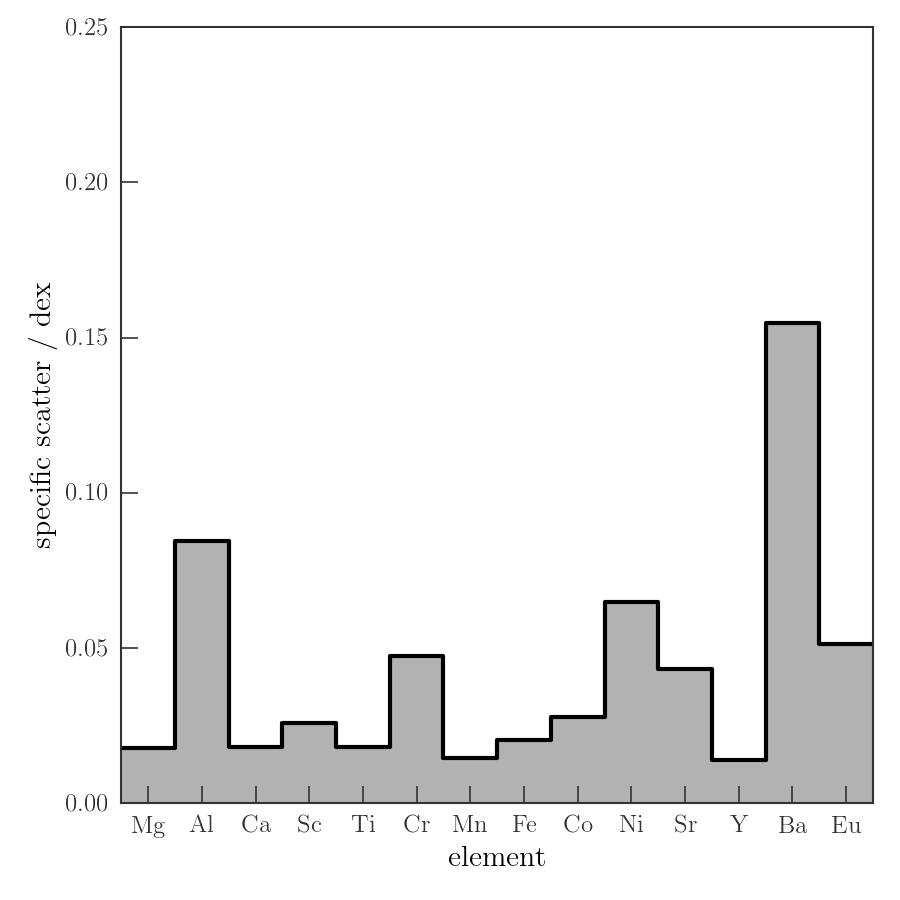
\includegraphics[width=0.45\textwidth]{experiments/exp2-specific-scatter.png}
	\caption{Specific scatter remaining in the \citet{Barklem:2005} data used in
			 Experiment~2 after accounting for the contributions by all latent
			 factors.}
    \label{fig:exp2-specific-scatter}
\end{figure}



\subsection{Experiment 4:\\Chemical abundances in the \Galah\ survey}
\label{sec:exp4}

In this experiment we perform blind chemical tagging using the 
photospheric abundances released as part of the second \Galah\ 
data release \citep{Buder:2018}. This data set includes
up to 23 chemical abundances reported for 342,682 stars.
Some abundances are not reported, for a variety of 
reasons related to astrophysics or the adopted analyses
(e.g., a star is too hot to estimate the abundance for a given
transition, or the signal-to-noise of the spectrum is too low).
Our method as described cannot handle missing data entries for
a given star, and as such we are forced to exclude stars that
do not have a full complement of abundances. However, we also
chose to exclude some elemental abundances from our chemical
tagging experiments. For example, our experiments
with \Galah\ data do not include lithium or carbon abundances because the
photospheric varies throughout a star's lifetime. This is true
to a small degree for many elements \citep[e.g.,][]{Dotter:2017},
but for the purposes of this experiment we assume that all other
photospheric abundances remain constant throughout  a star's
lifetime.

We first selected stars with \texttt{flag\_cannon = 0} to exclude
stars where there is reason to suspect that the stellar parameters
(e.g., $\teff$, $\logg$) are unreliable, and as a result the 
detailed chemical abundances are untrustworthy. We ordered the
list of chemical abundances by the number of reliable measurements,
which is shown in Figure~\ref{fig:exp4-abundance-counts}. The number of
independent abundance measurements (e.g., where there is no reason
to suspect a single abundance to be untrustworthy) is shown in black,
and the cumulative number of trustworthy abundances is shown in blue.
The cumulative line can be interpreted as the number of stars for
which the full set of elemental abundances (up until and including
the abundance on the x-axis) is reported. We chose to include the
18 most commonly reported abundances (up to and including Al),
leaving us with a sample of \todo{50,000} stars.
These elements are produced from multiple nucleosynthetic
pathways, and it is this subsample that we will use for 
our initial chemical experiment with \Galah\ data.



\begin{figure}
	\includegraphics[width=0.45\textwidth]{experiments/exp4-abundance-counts.png}
	\caption{The number of abundance measurements in the second
		     \Galah\ data release \citep{Buder:2018} where \texttt{flag\_cannon = 0}
		     and \texttt{flag\_<element> = 0}. The black line indicates the number
		     of reported measurements for a single element, and the blue line
		     indicates the number of stars where all elements leftward (inclusive)
		     are reported. The dashed vertical line indicates the top 18 reported
		     elemental abundances, which we use for Experiment~4.}
    \label{fig:exp4-abundance-counts} 
\end{figure}


We executed a grid search for the number of latent factors $\NumLatentFactors$
and the number of components $\NumComponents$ that were preferred by the data.
Starting with $\NumLatentFactors = 1$ and $\NumComponents = 1$, we trialled each
permutation of $\NumLatentFactors$ and $\NumComponents$ up until $\NumLatentFactors = \NumDimensions - 1 = 17$
and $\NumComponents = 20$. For each permutation we initialised the model randomly,
and continued expectation-maximization until a tolerance of $10^{-5}$ was achieved
in the log-likelihood. The results of this grid search are shown in Figure~\ref{fig:exp4-gridsearch-contours},
where we show the best log-likelihood found for each permutation, and the corresponding
BIC value. The lowest BIC value is found for $\todo{\NumLatentFactors = X}$ and
$\todo{\NumComponents = X}$, which we adopted as the preferred number of latent
factors and components.

\todo{
\begin{enumerate}
	\item Plot data with most likely associations? Just as [Fe/H] vs [Si/Fe]?
	\item Plot factor loads, after rotation.
	\item Plot latent space.
	\item Plot aspects of the clusters identified.
	\item Plot specific scatter compared to the typical reported errors?
\end{enumerate}
}



\section{Discussion} \label{sec:discussion}


%We have presented a novel approach to chemical tagging that incorporates
%latent factors common to all stars, and allows for clustering in the relative
%contributions of those factors. This is analogous to simultaneously
%inferring nucleosynthetic yields as part of chemical tagging. 

Earlier studies investigating the limitations of chemical tagging have shown
that the effective dimensionality of chemical abundance space is lower than
the number of reported abundances \citep[e.g. about 8,][]{Ting:2008}. 
This is expected. Theoretical models of stellar evolution and nucleosynthesis 
suggest that there are of order \todo{5} nucleosynthetic mechanisms that are
predominately responsible for the production of the $\sim$20 or so observed 
reported in those studies. As a consequence we can expect that the observed
chemical abundances are correlated in some way (e.g., by a linear combination
of a fewer number of nucleosynthetic pathways).  However, most approaches to
chemical tagging to date have assumed that the observed chemical abundances
are independent of each other \todo{\citep[e.g.,][]{who}}. Those inferences
will be biased by that assumption in a non-trivial way. This problem cannot be
resolved by simply lowering the number of abundances used for chemical tagging (e.g.,
down to something near the effective dimensionality), either, because those
chemical abundances are still produced by multiple pathways.

Here we have introduced a model to simultaneously account for the lower
effective dimensionality of chemical abundance space, and perform clustering
in that lower dimensional space. Although our model allows us to estimate
those latent factors that contribute to all stars, and cluster those stars by
their relative contributions from those factors, there are issues with the
model we adopt. The model we describe is very likely \emph{not} the correct
model to use to describe chemical abundances of stars. We require the latent
factors in our model to be mutually orthogonal to each other. This suggests
an astrophysical context where the mean nucleosynthetic yields (over all star
formation histories and stellar masses) of various
processes (e.g., $r$-process, $s$-process) are mutually orthogonal to each
other. Clearly this assumption is likely to be incorrect: the nuclear physics
of one environment where elements are produced  can be very different from
other environments, and there is no astrophysical constraint that those
latent factors should be mutually orthogonal.
A more flexible data-driven model of nucleosynthetic yields (as a function of mass,
stellar metallicity, and other factors) that does not require the latent
factors to be mutually orthogonal would be a worthy extension to this work.

There are other issues in our model that relate to our assumption of mutual
orthogonality. Even if nucleosynthetic yields were truely mutually orthogonal,
then the latent factors we infer are only \emph{identifiable} up until an
orthogonal basis. As we have seen in our experiments, the ordering and sign 
of the latent factors is not described \emph{a priori}. That means that we
must `assign' the latent factors we infer as being described by an astrophysical
process (e.g., the zeroth-latent factor is r-process). A more general limitation
of this is that the latent factors can be multiplied by some arbitrary rotation
matrix, leading to latent factor loads that are very different from what was
estimated by the model, but still lead to the exact same data (or log-likelihood,
or Kullback-Liebler divergence, etc). As a consequence, we can only `identify'
latent factors up until this rotation. We have sought to address this by constructing
rotation matrices where the entries each latent factor correspond to our expectations
from astrophysical processes (whilst remaining orthogonal), but here we are limited
by what astrophysical processes we are \emph{expected} to find.

This constrains our ability to identify new nucleosynthetic processes. For example,
let us consider a hypothetical situation where we would only expect there to be four 
nucleosynthetic processes that predominately contribute to the observed \GALAH\ abundances,
but in practice we found that the data are best explained (with high significance) with
five latent factors. We construct a rotation matrix where the first four latent factors
describe the mean nucleosynthetic processes we expect to find. What of the fifth latent
factor? We can constrain the possible values of the fifth latent factor conditioned on
the requirement that all factors remain mutually orthogonal, but one can imagine that
some (or perhaps many) elements have entries where the fifth latent factor can have
near-zero or zero entries. Even if the mean nucleosynthetic yields are mutually
orthogonal, there are scenarios that one can imagine where there is a limited amount
we can say with confidence about that new nucleosynthetic process.

Notwithstanding these issues, we have presented numerous experiments that demonstrate
that a latent factor model that allows for clustering in latent space can adequately
describe chemical abundance data. Our experiments with toy data (Experiment~1) reliably
finds the true number of latent factors and cluster components when we adopt an information-theoretic approach to the objective function (e.g., BIC or MML), and correctly estimates the latent
model parameters. When applied to chemical abundances measured from metal-poor stars 
(Experiment~2) we find that \todo{seven latent factors and two clusters are preferred by
the data.}

\todo{discussion of experimental results}

\todo{
\begin{itemize}
	\item at low metallicities how many factors do we prefer, and what can we
		  vaguely interpret these at?
	\item when we do that to large galah data sets, what is the number of factors
	\item clustering in galah
	\item clustering in apogee
\end{itemize}
}


\section{Conclusions} \label{sec:conclusion}

\acknowledgements
A.~R.~C. is supported in part by Australian Research Council
Discovery Project DP160100637.
The \GALAH\ survey is based on observations made at the Australian Astronomical Observatory, under programmes A/2013B/13,
A/2014A/25, A/2015A/19, A/2017A/18. We acknowledge the traditional owners of the land on which the AAT stands, the Gamilaraay
people, and pay our respects to elders past and present.
This work presents results from the European Space Agency (ESA) space mission Gaia. Gaia data is being processed by the Gaia Data Processing and Analysis Consortium (DPAC). Funding for the DPAC is provided by national institutions, in particular the institutions participating in the Gaia MultiLateral Agreement (MLA). The Gaia mission website is https://www.cosmos.esa.int/gaia . The Gaia archive website is https://archives.esac.esa.int/gaia .
This research has made use of NASA's Astrophysics Data System.


\software{
	\package{Astropy}\,\,\citep{astropy:v1,astropy:v2},\,\,
    \package{IPython}\,\,\citep{ipython},\,\,
    \package{matplotlib}\,\,\citep{mpl},\,\,
    \package{numpy}\,\,\citep{numpy},\,\,
    \package{scipy}\,\,\citep{scipy},\,\,
    \package{Stan}\,\,\citep{stan},\,\,
    \package{Jupyter Notebooks}\,\,\citep{jupyter-notebooks}\,\,
}    



\bibliographystyle{aasjournal}
\bibliography{mcfa}

\end{document}
